% This is LLNCS.DEM the demonstration file of
% the LaTeX macro package from Springer-Verlag
% for Lecture Notes in Computer Science,
% version 2.2 for LaTeX2e
%
\documentclass{llncs_Ibergrid2013}
%
\usepackage{makeidx}  % allows for indexgeneration
%
%\usepackage[dvips]{graphicx}
%
\usepackage{epsfig}
\usepackage{cite}
\usepackage{url}
\usepackage{microtype}
\usepackage[english]{babel}
\usepackage{graphicx}
\usepackage{eurosym}
\usepackage{url}
\usepackage{multirow}
\usepackage{listings}
\usepackage{natbib}
\begin{document}
%
\frontmatter          % for the preliminaries
%
\pagestyle{headings}  % switches on printing of running heads
\addtocmark{Federated Appliance Distribution in a Federated Cloud} % additional mark in the TOC
%
\mainmatter              % start of the contributions
%
\title{Federated Appliance Distribution in a Federated Cloud}
%
\titlerunning{VM Image Management}  % abbreviated title (for running head)
%                                     also used for the TOC unless
%                                     \toctitle is used
%
\author{A. Sim\'on\inst{1}, E. Freire\inst{1}, R. Rosende\inst{1}, I. D\'iaz\inst{1}, A. Feij\'oo\inst{1}, P. Rey\inst{1}, J. L\'opez-Cacheiro\inst{1}, C. Fern\'andez\inst{1} and O. Synge\inst{2}}
%
%\authorrunning{First Author et al.}   % abbreviated author list (for running head)
%
%%%% modified list of authors for the TOC (add the affiliations)
\tocauthor{First Author (Institution of first author's affiliation),
Second Author (Institution of second author's affiliation)}
%
\institute{Fundaci\'on Centro de Supercomputaci\'on de Galicia, Santiago de Compostela, Spain\\
\email{grid-admin@cesga.es}
\and
\email{owen.synge@jaysnest.de}
}




\maketitle              % typeset the title of the contribution

\begin{abstract}
With the development of Federated cloud infrastructures, Maintainers of virtual appliances need a mechanism to distribute their work to sites, ideally without external dependencies that may delay critical updates to virtual appliances. This paper summarises the work developed within EGI FedCloud taskforce during the last year to deploy a sustainable Federated Appliance life cycle Management System. This allows Appliance Maintainers to manage the life cycle of Appliances on the Federated services they use without the need for centralised resources or services.
\end{abstract}

%
\section{Introduction}
\label{sect-introduction}
%
With virtual appliances on Cloud IaaS resources the complications for integrating multiple components and dependencies of a service can be managed closer to the appliance creator or maintainer without need for the cloud resource provider to be involved. Cloud IaaS has shown great commercial success, so much so that new cloud software stacks are being developed, and many companies and research institutes are deploying these clouds for both public and private use. EGI-inspire brings together many sites, running multiple IaaS Cloud implementations as a Federated cloud. As part of this effort they are making efforts to help abstract away these differences so that Virtual Appliance users and maintainers can remain IaaS implementation and site neutral.

Interoperability of Appliance distribution is one of the first dependencies in the process, of creating a federated cloud. This paper is focused on some of the issues surrounding Virtual Appliance Image Management in a federated cloud environment following the HVWG's proposals.

A federated cloud using a heterogeneous cloud frameworks ecosystem (OpenStack, OpenNebula, WNoDES~\cite{wnodes}, etc). may be presented with corresponding APIs, Appliance formats, and different contextualisation mechanism for each cloud implementation. The tools used to evaluate the HVWG's proposals did not support any specific cloud infrastructures at the start of this process, so adaptors had to be developed for each IaaS System supported. So far OpenStack and  OpenNebula adaptors have been developed by members of the Federated Cloud Task Force.

%\subsection{User Services}

\section{Motivation}
\label{sect-motivation}
The primary goal of a EGI-federated cloud task force is to investigate the potential of IaaS Clouds as a revolutionary upgrade to Grid Computing's use ability. IaaS Clouds have been been deployed at many sites where they are actively used by communities that never succeeded with Grid Computation~\cite[?]. The EGI-federated cloud task force are a test bed evaluating policies and technology for production use.

Secondary goals include providing a unification of the IaaS resources, from a users experience and form resource sharing making for a quality of service to be extended beyond the capabilities of a financially constrained resource provider.

This is very similar to the goals of Grid computing but making use of IaaS platforms. IaaS platforms have succeeded in the Market, while Grid computing succeeded only for big science with very homogeneous workloads. It is the belief of the author that this is related to IaaS Clouds, having far greater flexibility for the Appliance Maintainer then the Grid Equivalent. The relatively new term DevOps is now common, in IT, and this person is often closely associated with the role of Appliance management.
%\begin{figure}[h!]
%\centering
%\includegraphics[width=60mm,angle=90]{./PSFIGs/user-services.eps}
%\caption{Use case in IBERGRID}\label{figUSER}
%\end{figure}

\section{Federated Appliance Management}
\label{sect-fedimagemanagement}

This paper focuses on appliance distribution, in a federated cloud following the HVWG's recommendations. The aim of the HVWG was to propose policies so resource providers have a way to control and mange Virtual Machine (VM) Image's provided by experiments,that need to execute in a trusted environment (similar to the current computing environment provided under Grid computing). These goals may no longer be appropriate as Cloud Technology has developed allowing greater support for untrusted images.

This paper examines our experiance of testing this proposed polidcy and the use of the available tools, and how they where extended to be used in the EGI-federatred cloud task force. The authors of this paper are members of the EGI-federatred cloud task force collaborating with a maintainer of a HVWG image list subscriber, and a former member of the Hepix Virtualisation Working Groups.
\section{Related Work}
\label{sect-relatedwork}
The use of Cloud infrastructures in science has been documented, and it is a very promising field, but integrating Clouds with the Grid is a challenge, as related on Dillon et al.~\cite{Dillon2010}. Goasguen et al.~\cite{Goasguen2012} presents the results of an internal production cloud service in CERN and suggestions to expand it to another Grid sites. Zhao et al.~\cite{Zhao2012} presents a infrastructure of a dozen computing sites using OpenNebula as the management solution. It concludes that Clouds are useful for science, but there are still performance issues to be resolved. Hoffa et al.~\cite{Hoffa2008} reached similar conclusions regarding cloud vs local deployments.

There are also many works that compare the different solutions for VM Management, like Xiaolong et al.~\cite{Xiaolong2012}, which compares OpenNebula and Openstack, and Laszewski et al.~\cite{Laszewski2012}, which does a more complete survey including Eucalyptus, Nimbus and some other solutions. The existence of numerous trade-offs and fragmented market for these tools motivated us to support cross-grid environments.

On the realm of security, our solution emphasises the authentication of users and the validation of VMs. There are other works on the area, but some, like Xi et al.~\cite{Xi2012} are concerned more with running trusted VMs on on untested environments, which can be seen as the opposite problem, and many others, like Schwarzkopf et al.~\cite{Schwarzkopf2012} are concerned with improving the internal security of VMs maintained by Cloud users instead of infrastructure operators.

There are still other comparable solutions, Lagar-Cavilla et al.~\cite{Lagar-Cavilla2009} use a non-local fork mechanism to spawn many copies of a VM across many sites, but this method would be at odds with current Grid practices. Diaz et al.~\cite{Diaz2012} have a similar system that bridges OpenNebula and OpenStack, but it uses the Amazon EC2 API, which has licensing issues preventing us for using it, and does not address the authorisation and validation of VMs. On a more partial resemblance, Maurer et al.~\cite{Maurer2013} also automates some aspects of VM management and updates using an autonomous system, and Django et al.~\cite{Django2013} changes the context of VMs on the fly to do load balancing and improve brokering. This last functionality would be invaluable for Grid operators, which must frequently tend to processes that get stuck due to unrealistic brokering requirements, and would also avoid many down times due to reconfiguration.

\section{Appliance Lifecycle Management using Imagelists.}
\label{sect-appliancelifecycle}
The HVWG proposed a message system to decouple appliance maintainers from cloud implementations, this decoupling could be used to hide the heterogeneous nature of a federated cloud. The HVWG proposal are based upon SMIME and so is neutral of the method of signing and is applicable to pgp or x.509 signatures.

Imagelists are polled by the subscribers, their signature checked, image downloaded and the validity as an appliance checked using the secure hash. If the appliance image is valid the appliance is then able to be contextualised and then instantiated (see figure \ref{fig:infrastructure}). 
Using this mechanism a virtual image can be checked for validity, all image lists are signed and it provide a version number and expiration date. If the image list does not satisfy these requirements the image is not instantiated and the request is rejected.

The HVWG's subscription is similar to Debian's \textit{aptitude} or the rpm update management \textit{yum} utilities or a podcast subscriber. Publishing is similar to \textit{create-repo} which publishes rpm packages rather than virtual machines Appliances. But 2 major differences exist in the HVWG's proposals, that each image is uniquely identified by a UUID, and that Appliance image no longer present in an image list indicates their expiry of an appliance rather than an error as it would with package management.
\begin{figure}[h]
\centering
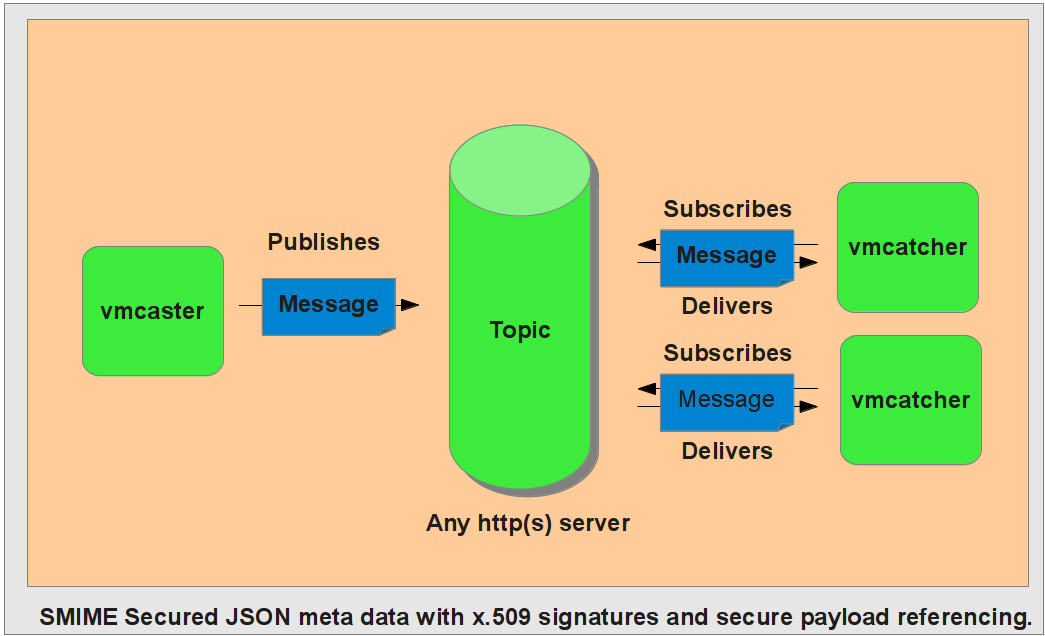
\includegraphics[width=1\textwidth]{vmcaster_vmcatcher.png}
\caption{VMcaster and VMcatcher infrastructure.}
\label{fig:infrastructure}
\end{figure}

\subsection{Publishing image lists}
Publishing images according to the HVWG's proposals is as simple as generating the meta data and signing it with standards SMIME signature routines. No new software is needed for this task. Due to the amount of meta data recommended by the HVWG and the expectation that users may want to add their own additional meta data, it is expected that users will use tools for generating the necessary JSON 

HVWG image lists use a JSON meta data file signed with SMIME and referencing images with secure hash seems an appropriate interface for the Appliance maintainer. However the amount of meta data recommended by the HVWG is burdensome to enter by hand.
 
VMcaster~\cite{vmcaster} is the 3rd iteration of increasingly automated image list publication tools. It was released after the EGI federated Cloud taskforce started using the HVWG's recommendations as VMcaster~\cite{vmcaster} automates the process of uploading images and Imagelists, to a greater level than previous tools and so was favoured by publishers. VMcaster~\cite{vmcaster} a generates as much meta data as possible from its local database, and the images while they are available, prior to upload.

\subsection{Subscribing to image lists}
VMcatcher~\cite{vmcatcher} is currently the only HVWG image list subscriber, and only supports JSON meta data and x509 signatures. Since the Grid community already use the International Grid Trust Federation~\cite{igtf} supporting just x.509 is acceptable for the current stage for the Federated cloud task force so these limitations nave not hindered this investigation. It is recommended that future HVWG image list providers support pgp and x.509 signatures.

vmcatcher allows subscription of virtual machine images by UUID so that a resource provider can provide contextualised appliance images from the most recent appliance image. Resource providers can configure their own image lists and select images from an image list, these are then validated in compliance with the Hepix security policies and cached locally. vmcatcher does not support any cloud explicitly so further work was needed in this area.

VMcaster can be configured to launch applications on image status change events such as expiry or new images becoming available. The federated Cloud task force has developed such integration handlers for managing Appliance Life cycle management with Open Stack and Open Nebula.
\section{Image management event handlers}
\label{sect-handlers}
\begin{figure}[h]
\centering
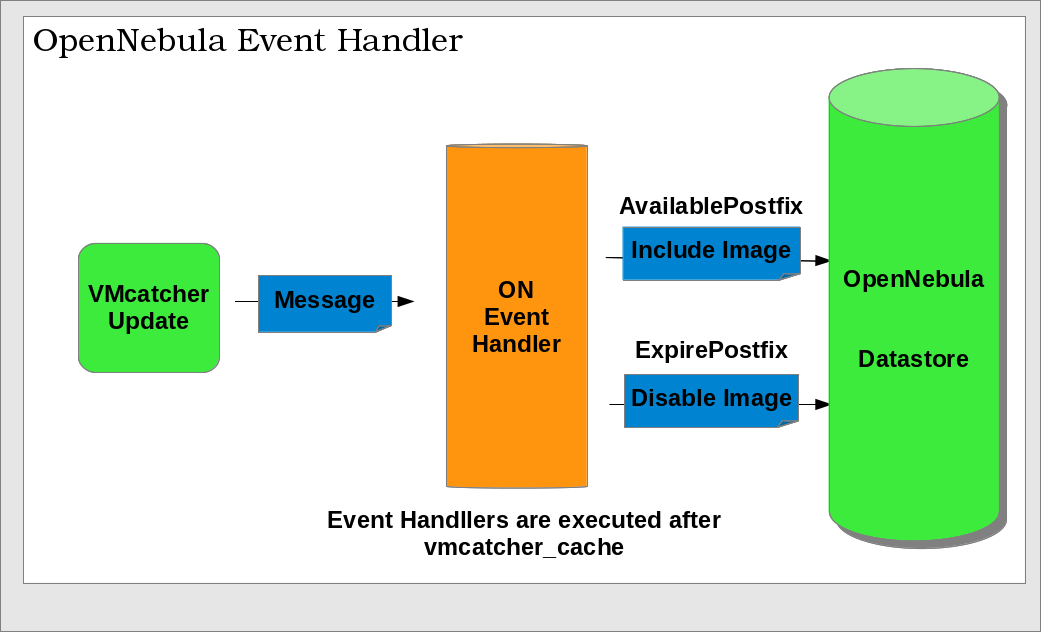
\includegraphics[width=1\textwidth]{ONeventhandler.png}
\caption{OpenNebula event handler.}
\label{fig:onevent}
\end{figure}
OpenNebula event handler~\cite{onevent} was developed by the CESGA team and currently is available from the VMcaster repository. 
The \textit{vmcatcher\_eventHndlExpl\_ON} package provides a new python and cron script which detects VMcatcher events. 
This script detects several VMcatcher event types. In this case OpenNebula handler only waits for a new Expire or Available VMcatcher event.
If VMcatcher raises a \textit{AvailablePostfix} event, this is detected by \textit{vmcatcher\_eventHndlExpl\_ON} event handler and reads the new image attributes such UUID, image name, description and image format.

If a new image is downloaded (\textit{AvailablePostfix} event), the OpenNebula event handler gets the image information, generates a new OpenNebula template and includes the new image into the local OpenNebula data store (see figure \ref{fig:onevent}). 
For security reasons, the new images are not public, they are only available for the oneadmin user. The OpenNebula administrator should verify the new image first (checking its contextualisation script, if the image is executed correctly etc).
After this period of time the image status is changed to be available for external users. 
Moreover if VMcatcher detects an image revocation the OpenNebula event handler search the image UUID from OpenNebula image database and it is set to disable status.
The image is not removed by the event handler, it should be removed by the site administrator from the OpenNebula datastore.

The OpenNebula event handler is not the only one. OpenStack administrators can also use Glancepush~\cite{glancepush} service to keep their local image catalogue updated. 
This service was developed at IN2P3 and it works in a similar way than the OpenNebula event handler. 
In this case Glancepush updates the OpenStack Image Service (Glance) if it detects any image change from VMcatcher tool. 
The new package (\textit{glancepush-vmcatcher}) is available from IN2P3 ftp server, and it only requires a working glance service and an OpenStack user account to push images into the catalogue.

%\section{Use Case: EGI SA2.3 verification image repository}
%\label{sect-usecase}
%This is my text 


\section{Results from long term testing the HVWG proposals as a Federated Apliance mangement framework}
\label{sect-experiances}
The HVWG's polices where tested to allow this distributed model, requires appliance maintainers, to allow images to be executed at a set of sites rather than contact each individually. With these tools we tried to match the requirements set by the now completed HEPiX Virtualisation working group~\cite{hepix}.

During the last year the EGI federated cloud task force has recommended VMcatcher as well for installation at all cloud resource providers in their collaboration and the status of the integration with OpenStack and OpenNebula.

As demonstrated in the Federated Cloud Demo (we need a citation), HVWG proposals and the implementations vmcatcher and vmcaster worked successfully and are relatively east to deploy and configure. Investigation shows they operate without a single point of failure. Fully automated image updates between more than one site in both directions have been shown to work. on both Open Stack and Open Nebuala using the handelrs developed by the Federated Cloud force. Combined with the Hepix security policy, the appliance management system in testing has shown itself to be a basis of a full automated, federated image distribution system in practice and currently production grade.

Long term testing and practice has shown that not all appliance producers regularly upgrade their images. If appliance maintainers do update it is unusual that they do so at the frequency expected by the Hepix Virtualisation working groups policies. By providing greater isolation at the network level, NIKEF and Oxford University in particular, have long suggested that they are able to run insecure images, without fear of appliances negatively effecting each other. CESGA is planing on developing policies and practices to also achieve this in the future.

In light of the flexibility allowed by greater network isolation, the monthly update recommendations from the Hepix Virtualisation Working group now seem overly optimistic. The flexibility in Cloud networking capabilities where not for seen in the Hepix proposals and consequently the ability to run potentially outdated Appliances in a secured networking environment, where not addressed by the HVWG.

\section{Continued use outside the Federated cloud taskforce}
\label{sect-continued}

A new use cases is the EGI SA2.3 verification image repository. The EGI SA2 test-bed is used to verify and test the new middle ware before reaching the production software repository (UMD).
One of the most important new features is the ability to distribute and publish VM images in an automated way. 
These new tools, like EGI MarketPlace\footnote{EGI MarketPlace: \url{http://marketplace.egi.eu}} and VMcatcher\footnote{VMcatcher: \url{https://github.com/hepix-virtualisation/vmcatcher}} can be also used within SA2 verification process to distribute and publish new UMD services after its verification. 
This work is still on going and it will be available in the next months. Using this infrastructure the new EGI certified image it will be available to be used and tested by EGI site administrators after each successful verification.

For the moment after each software verification the images are stored locally within CESGA's OpenNebula datastore but using VMcaster the new images will be published in an automated way.
This new paradigm will be useful for users that want to check the latest software changes without the need to install a new service from scratch.
Fortunately as we have explained in this paper, VMcatcher is not tightly coupled to any cloud framework to distribute and update images so images can be imported into the customers tools of choice. The new image management tools are being used by EGI Fedcloud providers since last year successfully and it is expected more use cases in the near future will be solved using this set of tools.

\section{Conclusions and Future work}
\label{sect-conclusions}
The greatest potential for the EGI-federatred cloud task force is to simplify the management of IaaS systems over the native API's. However Cloud implementation neutrality increases the Interoperability challenges. 
The HVWG propsal was esentially federated with a distributed system, with no single point of failure or single service in control, and with a policy that was agreed by the mebers of the HVWG.

The use of a simple signed lists of endorsed Appliances in the HVWG proposals is equally applicable to all PKI infrastructures supported by SMIME. The implementation called vmcatcher is not so flexible but the limitations have not hindered this investigation.

We believe that the HVWG proposal to manage Appliance Lifecycle, with signed messages listing Appliances that are valid is expressive enough for federating appliances. Appliance management is typically IO bound and so asynchronous in nature signed images list provide a simple and clear way of managing appliance images are checked by resource providers. We found the clear definition of valid and invalid/expired images, and the distributed nature of Appliance lists a natural fit to a federated cloud and worth testing.

Having tested the use of Hepix proposed image distribution system, with the tools vmcatcher, vmcaster and having developed event handlers, the Federated Cloud Task force have proved this approach is a distributed system for image distribution, to Open Stack and Open Nebuala resource providers. The Fedcloud task force have validated VMcaster and VMcatcher utilities as production grade implementation of the HVWG's recommendations, and will continue to be uses them to distribute and validate VM images.

The policies proposed by the HVWG seem overly restrictive for the Federated Cloud. It should be noted that the both the Imagelists and image meta data can be extended to support extra meta data and pass this meta data through the vmcaster and vmcatcher infrastructure. This could be used to reference a variety of Policies used to federate images between sites should such policies be developed. We recomend that the EGI Fed Cloud task force develops a variety of update policies applicable to a wider range of both sites and user communities than proposed by the HVWG. Greater network isolation between Appliances from different customers allowing support of potentially outdated and poorly supported Appliance has changed the posisbilities for policy development.

For these reasons we consider that the proposals provided by the Hepix Virtualisation working group as a useful starting point for the EGI Federated Cloud task force and the implementation is production grade. We recommend that the policies are updated to reflect differing levels of network isolation available at sites within the EGI federated cloud at sites in the Federated cloud task force.

\section*{Acknowledgements}
\label{sect-acknowledgements}
This work is partially funded by the  EGI-InSPIRE (European Grid Initiative: Integrated Sustainable
Pan-European Infrastructure for Researchers in Europe) is a project co-funded by the European Commission 
(contract number INFSO-RI-261323) as an Integrated Infrastructure Initiative within the 7th Framework 
Programme. EGI-InSPIRE began in May 2010 and will run for 4 years. Full information is available at:
\url{http://www.egi.eu/}.

%
% ---- Bibliography ----
%
%\begin{thebibliography}{99}
%
\bibliographystyle{abbrv}

%\bibliographystyle{thebibliography}
\bibliography{bibliography}

%\bibitem{dcache}
%\newblock The dcache book. 
%\newblock \url{http://www.dcache.org/manuals/Book/}, May 2013.


%\bibitem{Django2013}
%\newblock D. Armstrong et al.
%\newblock Runtime virtual machine recontextualization for clouds.
%\newblock Euro-Par 2012: Parallel Processing Workshops. Volume 7640 of Lecture Notes in Computer Science, pages 567--576. Springer Berlin Heidelberg, 2013.

%\bibitem{hepix}
%T.~Cass.
%\newblock The hepix virtualisation working group: Towards a grid of clouds.
%\newblock {\em Journal of Physics: Conference Series}, 396(3):032020, 2012.

%\bibitem{Diaz2012}
%J.~Diaz, G.~von Laszewski, F.~Wang, and G.~Fox.
%\newblock Abstract image management and universal image registration for
%  {C}loud and {HPC} infrastructures.
%\newblock In {\em Cloud Computing (CLOUD), 2012 IEEE 5th International
%  Conference on}, pages 463--470, 2012.

%\bibitem{Dillon2010}
%T.~Dillon, C.~Wu, and E.~Chang.
%\newblock Cloud computing: Issues and challenges.
%\newblock In {\em Advanced Information Networking and Applications (AINA), 2010
%  24th IEEE International Conference on}, pages 27--33, 2010.

%\bibitem{Lagar-Cavilla2009}
%L.-C. et~al.
%\newblock Snowflock: rapid virtual machine cloning for cloud computing.
%\newblock In {\em Proceedings of the 4th ACM European conference on Computer
%  systems}, EuroSys '09, pages 1--12, New York, NY, USA, 2009. ACM.

%\bibitem{Goasguen2012}
%S.~Goasguen, B.~Moreira, E.~Roche, and U.~Schwickerath.
%\newblock Lxcloud : a prototype for an internal cloud in hep. experiences and
%  lessons learned.
%\newblock {\em Journal of Physics: Conference Series}, 396(3):032098, 2012.

%\bibitem{Hoffa2008}
%C.~Hoffa, G.~Mehta, T.~Freeman, E.~Deelman, K.~Keahey, B.~Berriman, and
%  J.~Good.
%\newblock On the use of cloud computing for scientific workflows.
%\newblock In {\em eScience, 2008. eScience '08. IEEE Fourth International
% Conference on}, pages 640--645, 2008.

%\bibitem{Xi2012}
%C.~Li, A.~Raghunathan, and N.~Jha.
%\newblock A trusted virtual machine in an untrusted management environment.
%\newblock {\em Services Computing, IEEE Transactions on}, 5(4):472--483, 2012.

%\bibitem{Maurer2013}
%M.~Maurer, I.~Brandic, and R.~Sakellariou.
%\newblock Adaptive resource configuration for cloud infrastructure management.
%\newblock {\em Future Generation Computer Systems}, 29(2):472 -- 487, 2013.

%\bibitem{glancepush}
%M.~Puel.
%\newblock Openstack glancepush service.
%  \url{https://github.com/EGI-FCTF/glancepush/wiki}, 2013.

%\bibitem{onevent}
%R.~Rosende.
%\newblock Opennebula event handler.
%  \url{https://github.com/grid-admin/vmcatcher\_eventHndlExpl\_ON}, May 2013.

%\bibitem{wnodes}
%D.~Salomoni, A.~Italiano, and E.~Ronchieri.
%\newblock Wnodes, a tool for integrated grid and cloud access and computing
%  farm virtualization.
%\newblock {\em Journal of Physics: Conference Series}, 331:052017, 2011.

%\bibitem{Schwarzkopf2012}
%R.~Schwarzkopf, M.~Schmidt, C.~Strack, S.~Martin, and B.~Freisleben.
%\newblock Increasing virtual machine security in cloud environments.
%\newblock {\em Journal of Cloud Computing}, 1(1):1--12, 2012.

%\bibitem{vmcaster}
%O.~Synge.
%\newblock Vmcaster vm image publication tool.
%  \url{https://github.com/hepix-virtualisation/vmcaster}, May 2013.

%\bibitem{vmcatcher}
%O.~Synge.
%\newblock Vmcatcher image subscription tool.
%  \url{https://github.com/hepix-virtualisation/vmcatcher}, May 2013.

%\bibitem{Laszewski2012}
%G.~von Laszewski, J.~Diaz, F.~Wang, and G.~Fox.
%\newblock Comparison of multiple cloud frameworks.
%\newblock In {\em Cloud Computing (CLOUD), 2012 IEEE 5th International
%  Conference on}, pages 734--741, 2012.

%\bibitem{Xiaolong2012}
%X.~Wen, G.~Gu, Q.~Li, Y.~Gao, and X.~Zhang.
%\newblock Comparison of open-source cloud management platforms: Openstack and opennebula.
%\newblock In Fuzzy Systems and Knowledge Discovery (FSKD), 2012 9th
%\newblock  International Conference on, pages 2457--2461, 2012.

%\bibitem{Zhao2012}
%Y.~Zhao, Y.~Zhang, W.~Tian, R.~Xue, and C.~Lin.
%\newblock Designing and deploying a scientific computing cloud platform.
%\newblock In {\em Grid Computing (GRID), 2012 ACM/IEEE 13th International
%  Conference on}, pages 104--113, 2012.

%\end{thebibliography}


\end{document}
